\documentclass{article}
\usepackage{amsmath}
\usepackage{mathtext}
\usepackage[T1,T2a]{fontenc}
\usepackage[utf8]{inputenc}
\usepackage[english, bulgarian, russian]{babel}
\usepackage{tikz}
\usepackage{pgfplots}
\usepackage[export]{adjustbox}
\usepackage{siunitx}
\usepackage{booktabs}
\usepackage{pgfplotstable}
\usepackage[left=2cm,right=2cm,
    top=2cm,bottom=2cm,bindingoffset=0cm]{geometry}
    
    
\sisetup{
  round-mode          = places, % Rounds numbers
  round-precision     = 2, % to 2 places
}

\title{Лабораторная работа 1.4.5\\Изучение колебаний струны}
\date{6 декабря 2019}
\author{Стрижак Даниил}

\begin{document}
  \pagenumbering{gobble}
  \maketitle
  \newpage
  \pagenumbering{arabic}
  
  

\section{Аннотация}

В работе изучается явление поперечных стоячих волн в струне: определяются собственные частоты колебаний струны в зависимости от натяжения струны и определение скорости распространения поперечных волн в струне с помощью звукового генератора, двухканального осциллографа, частотомера, набора грузов и станины, с закрепленной на ней струной.


\section{Теоретические сведения}

Стоячая волна возникает в результате интерференции и представляет собой колебательный процесс с
устойчивым в пространстве расположением максимумов (пучностей) и минимумов (узлов).
Колебания ограниченной, закрепленной на концах струны, являющиеся стоячими волнами задаются
уравнением:

\begin{equation*}
  \frac{\delta^2y}{\delta t^2} = - u^2\frac{\delta^2y}{\delta x^2},\\	
\end{equation*}
где:

\begin{equation}
  u= \sqrt{\frac{T}{\rho_l}}.\\	
\end{equation*}

Так как на концах струны амплитуда колебаний равна нулю, в струну длиной L должно укладываться целое число полуволн:

\begin{equation*}
  L = \frac{\lambda_n}{2}n.\\	
\end{equation*}

Поскольку длина волны однозначно связана с ее частотой, стуна может колебаться только с определенными частотами:

\begin{align*}
  \nu_n = \frac{u}{\lambda_n}=\frac{n}{2L}\sqrt{\frac{T}{\rho_l}}, \ n \in \mathbb{N}.\\	
\end{align*}

Набор таких частот называют собственными частотами колебаний струны. 

\begin{center}

  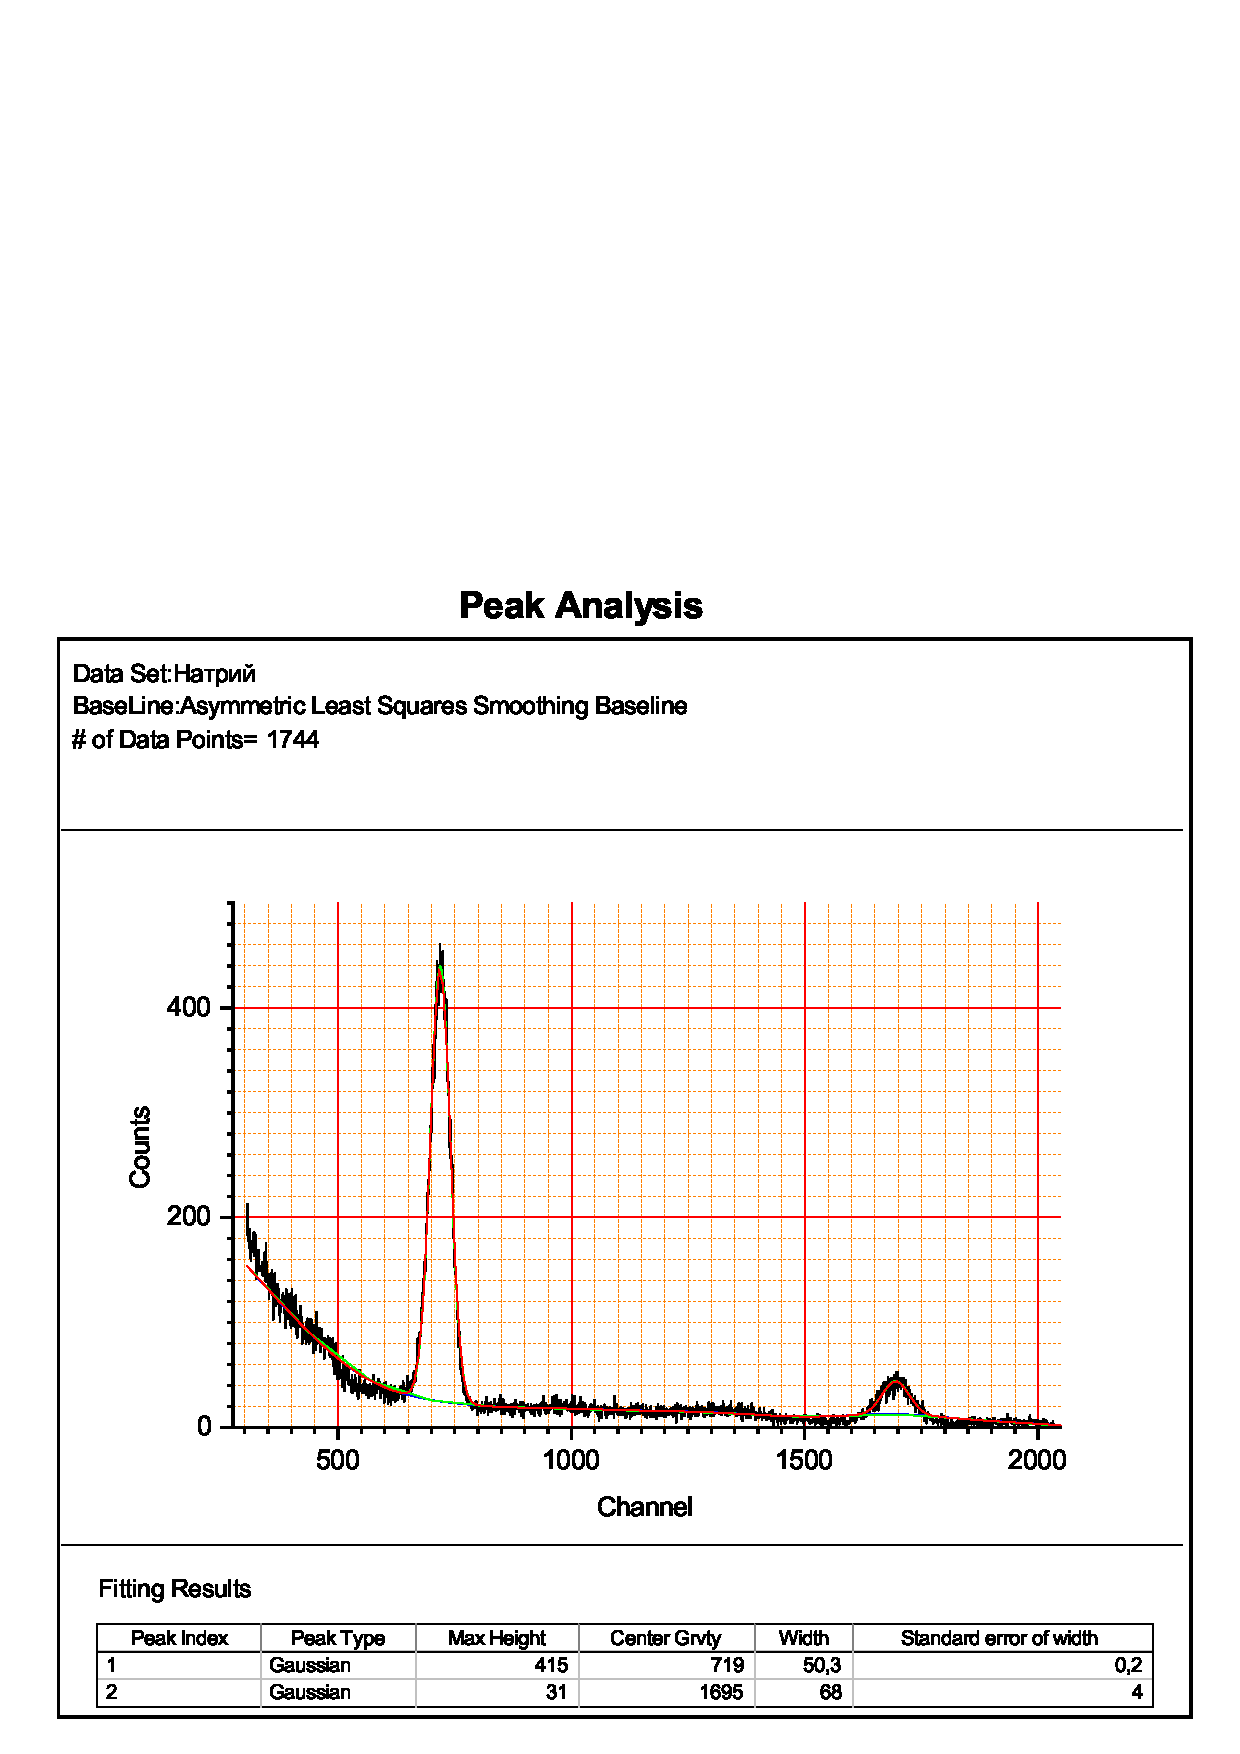
\includegraphics[width=0.5\linewidth]{1.jpeg}\\
 
   Стоячие волны (собственные моды колебаний струны) для n = 1,2,3\\
 
 \end{center}


Резонанс возникает при совпадении внешней синусоидальной силы с частотой собственных колебаний
пружины.Струна возбуждается синусоидальным сигналом от генератора при помощи датчика у конца струны. Сигнал в катушке , которая находится в пучности, регистрируется осциллографом.




\section{Оборудование и инструментальные погрешности}

В работе используются: звуковой генератор, двухканальный осциллограф, частотомер, набор грузов, станина,с закрепленной на ней струной.\\
\\
1. Точность измерения массы грузов -- 0,1 г. \\
2. Точность измерения с помощью линейки -- 0,5 мм. \\
3. Точность измерения частот -- 0,1 Гц. \\

\section{Результаты измерений и обработка данных}
\subsection{Подготовка к эксперименту}
Схема экспериментальной установки:

\begin{center}

  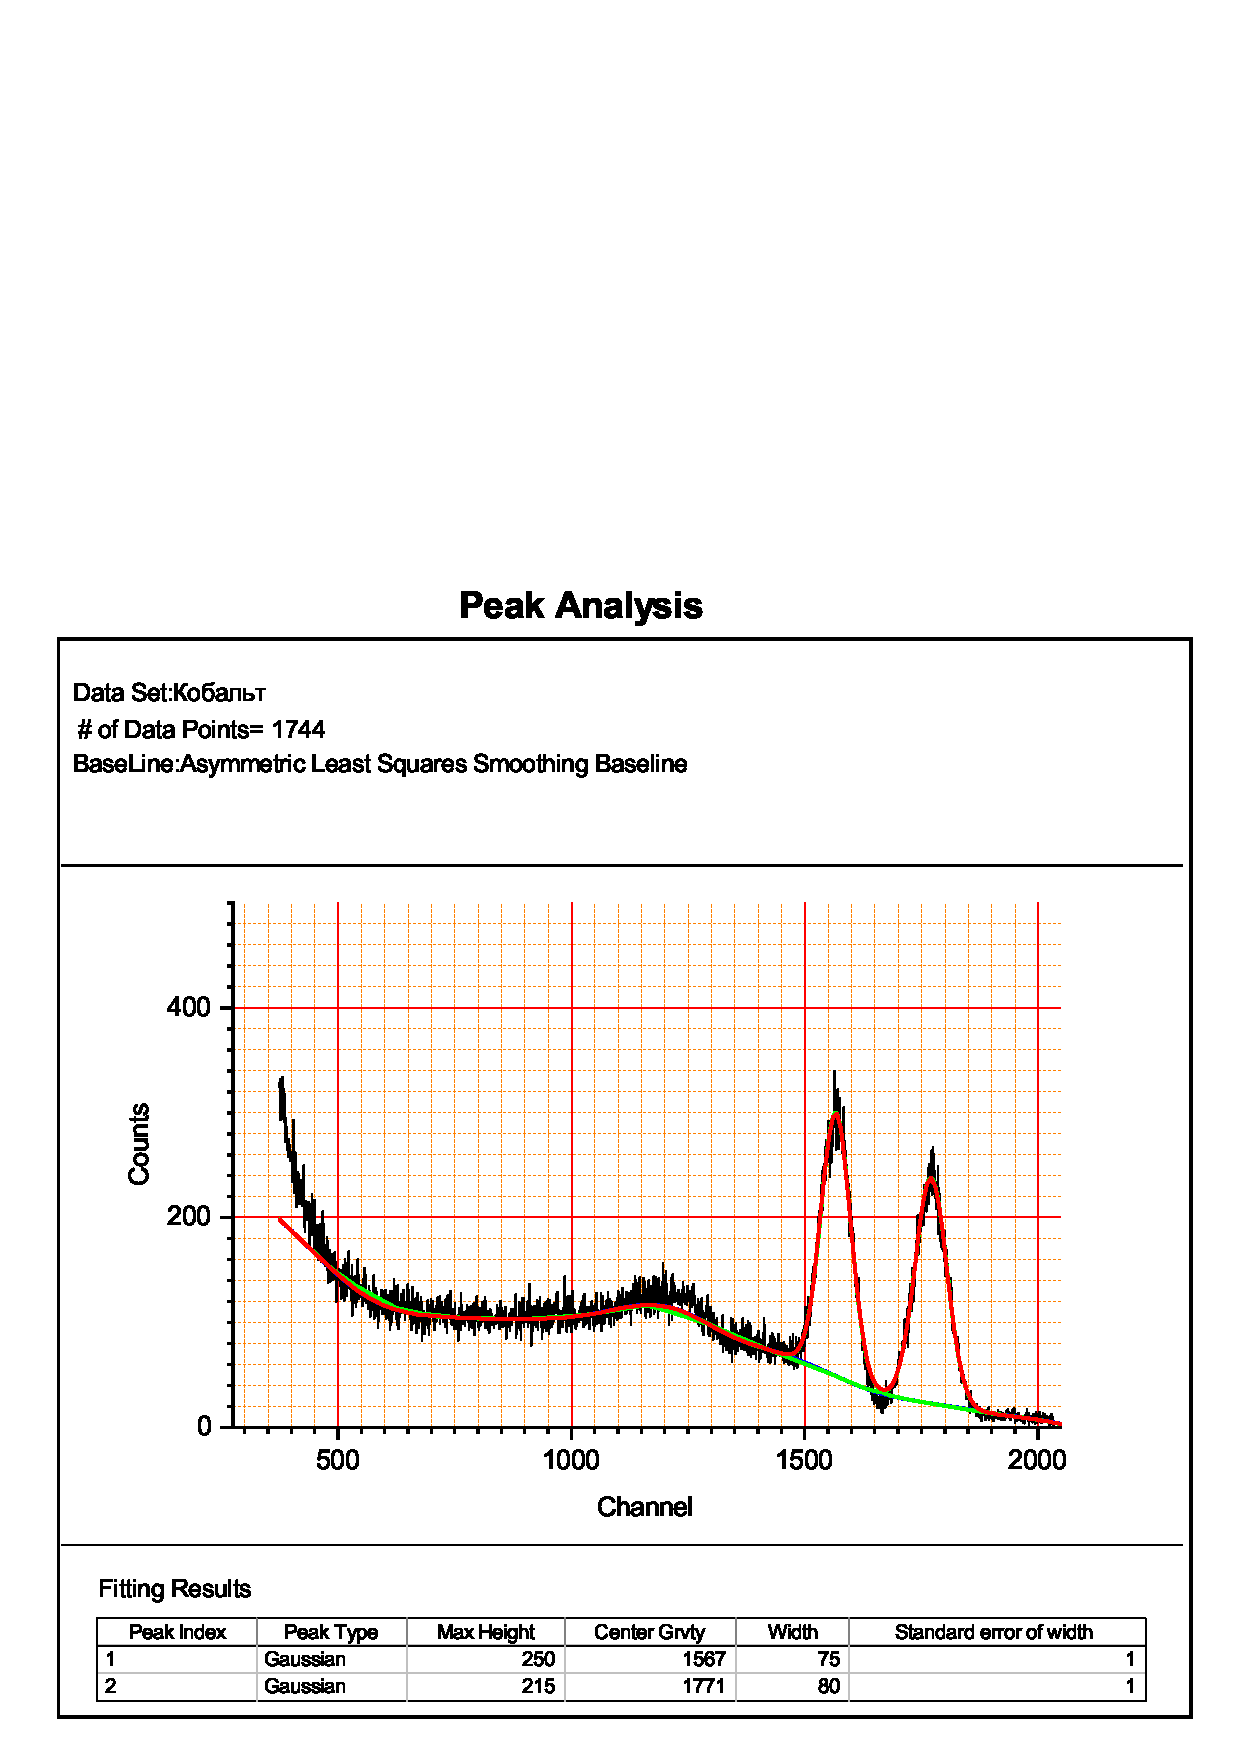
\includegraphics[width=0.8\linewidth]{2.jpeg}\\
 
   \\
 
 \end{center}
 
1. Освободим зажим струны на стойке 3, установим длину струны L = 50 см. Натянем струну, поставив на платформу грузы (примерно 0,5 кг) (учитывая вес платформы и крепежа). Осторожно зажмем струну в стойке, не деформируя струну. Возбуждающий датчик 6 должен располагаться рядом с неподвижной
стойкой 2, т.е. вблизи узла стоячей волны.

\\



2. Проведем предварительные расчёты. Оцените скорость распространения волн,  используя табличное значение плотности стали и приняв диаметр струны равным d $\approx$ 0,3 мм. Для заданных значений длины струны и силы натяжения рассчитаем частоту основной гармоники $\nu_1$ согласно формулам, написанным выше.

\begin{align*}
  u&=110\pm2 \ \frac{м}{с}, \\
\end{align*}

3. Включим в сеть звуковой генератор и частотомер. Установим на генераторе тип сигнала — синусоидальный, частоту основной гармоники $\nu_1$ и максимальную амплитуду напряжения. При этом сигнал с выхода генератора должен быть подан на возбуждающий датчик 6 (проверим правильность соединения проводов!).

\newpage
\subsection{Наблюдение стоячих волн прямым наблюдением}
1. Медленно меняя частоту звукового генератора в диапазоне $\nu =\nu_1 \pm 5$Гц, добьемся возбуждения стоячей волны на основной гармонике (одна пучность). Если при колебаниях струна касается регистрирующего датчика 8, осторожно сдвинем датчик по скамье в сторону подвижного зажима струны 3. Определим частоту первой гармоники по частотомеру.
2. Увеличив частоту в 2 раза, получим картину стоячих волн на второй гармонике, а затем и на более высоких гармониках. 

\begin{center}
	\begin{tabular}{|c|c|}
		\hline
 		$№$ & $\nu, \ Гц$   \\
		\hline 
		1 & 100,6 \\
		\hline
		2 & 205,8 \\
		\hline 
 		3 & 305,4\\
		\hline
 		4 & 413,2 \\
		\hline
 		5 & 515,3\\
		\hline
		6 & 620,9 \\
		\hline
		7 & 726,0\\
		\hline
	\end{tabular}
\end{center}


\subsection{Регистрация стоячих волн с помощью осциллографа}\\

1. Визуально настроем струну на основной гармонике, не меняя нагрузку струны и её длину. Установим регистрирующий датчик 8 в центре под струной (в пучности стоячей волны). Уменьшим уровень выходного сигнала генератора так, чтобы при колебаниях струна не касалась датчика. Проверим правильность соединения проводов. \\

2. Включим осциллограф в сеть и проверим его настройку.
Подстроим частоту генератора так, чтобы амплитуда сигнала была максимальна. Добьемся отсутствия нелинейных искажений, уменьшая уровень возбуждения (амплитуду напряжения генератора) и подстраивая при этом частоту так, чтобы она соответствовала максимуму сигнала. 

\begin{center}
  \begin{minipage}{0.15\textwidth}
	\begin{tabular}{|c|c|}
	  \hline
 		$№$ & $\nu, \ Гц$   \\
		\hline 
		1 & 100,6 \\
		\hline
		2 & 205,8 \\
		\hline 
 		3 & 305,4\\
		\hline
 		4 & 413,2 \\
		\hline
 		5 & 515,3\\
		\hline
		6 & 620,9 \\
		\hline
		7 & 726,0\\
		\hline
		8 & 830,3\\
		\hline
		9 & 930,9 \\
		\hline
		10 & 1033,4\\
		\hline
	\end{tabular}
	\begin{center}
	  \caption{Нагрузка \\  6,89 Н}
	\end{center}
  \end{minipage}
  \begin{minipage}{0.15\textwidth}
	\begin{tabular}{|c|c|}
	  \hline
 		$№$ & $\nu, \ Гц$   \\
		\hline 
		1 & 129,3\\
		\hline
		2 & 258,4 \\
		\hline 
 		3 & 388,1\\
		\hline
 		4 & 523,6 \\
		\hline
 		5 & 651,2\\
		\hline
		6 & 783,3 \\
		\hline
		7 & 915,2\\
		\hline
		8 & 1050,1\\
		\hline
		9 & 1184,0\\
		\hline
		10 & 1322,0\\
		\hline
	\end{tabular}
	\begin{center}
	  \caption{Нагрузка \\ 10,24 Н}
	\end{center}
  \end{minipage}
  \begin{minipage}{0.15\textwidth}
	\begin{tabular}{|c|c|}
	  \hline
 		$№$ & $\nu, \ Гц$   \\
		\hline 
		1 & 158,6 \\
		\hline
		2 & 313,2 \\
		\hline 
 		3 & 469,4\\
		\hline
 		4 & 629,2 \\
		\hline
 		5 & 786,1\\
		\hline
		6 & 944,1 \\
		\hline
		7 & 1102,1\\
		\hline
		8 & 1264,1\\
		\hline
		9 & 1423,3\\
		\hline
		10 & 1586,5\\
		\hline
	\end{tabular}
	\begin{center}
	  \caption{Нагрузка \\ 15,03 Н}
	\end{center}
  \end{minipage}
  \begin{minipage}{0.15\textwidth}
	\begin{tabular}{|c|c|}
	  \hline
 		$№$ & $\nu, \ Гц$   \\
		\hline 
		1 & 182,0 \\
		\hline
		2 & 365,8 \\
		\hline 
 		3 & 549,8\\
		\hline
 		4 & 733,4 \\
		\hline
 		5 & 916,0\\
		\hline
		6 & 1100,3 \\
		\hline
		7 & 1286,0\\
		\hline
		8 & 1472,5\\
		\hline
		9 & 1658,4\\
		\hline
		10 & 1847,2\\
		\hline
	\end{tabular}
	\begin{center}
	  \caption{Нагрузка \\ 19,75 Н}
	\end{center}
\end{minipage}
\begin{minipage}{0.15\textwidth}
	\begin{tabular}{|c|c|}
	  \hline
 		$№$ & $\nu, \ Гц$   \\
		\hline 
		1 & 205,0 \\
		\hline
		2 & 410,2 \\
		\hline 
 		3 & 616,2\\
		\hline
 		4 & 821,9 \\
		\hline
 		5 & 1028,4\\
		\hline
		6 & 1232,2\\
		\hline
		7 & 1441,1\\
		\hline
		8 & 1647,6\\
		\hline
		9 & 1861,3\\
		\hline
		10 & 2062,0\\
		\hline
	\end{tabular}
	\begin{center}
	  \caption{Нагрузка \\ 24,48 Н}
	\end{center}
  \end{minipage}
\end{center}

\newpage
Графики зависимости частоты от n представлены ниже:

\begin{center}

  \includegraphics[width=0.8\linewidth]{task.png}\\
 
   \\
 
 \end{center}

Из графиков имеем зависимость u от T:\\

\begin{center}
\begin{tabular}{|c|c|c|}
	  \hline
 		$T, H$ & $u, \ \frac{м}{с}$ & $u^2, \ \frac{м^2}{с^2}$   \\
		\hline 
		6,89 & 103,06 & 10621 \\
		\hline
		10,24 & 130,69 & 17080 \\
		\hline 
 		15,03 & 157,5& 24806\\
		\hline
 		19,75 & 183,64& 33724 \\
		\hline
 		24,48 & 205,8& 42353\\
		\hline
	\end{tabular}
\end{center}

\begin{center}
\begin{tikzpicture}[scale = 1.2]
\begin{axis}[
    axis lines = left,
    legend style={at={(0.8,1)}},
    xlabel = {$T, H$},
    ylabel = {$u^2, \ \frac{м^2}{с^2} $},
    xmin=6.5, xmax=25,
    ymin=10000, ymax=42500,
	ymajorgrids = true,
	xmajorgrids = true
]
\addplot[
	mark = square, 
	mark options = {
		scale = 1.5, 
		fill = red, 
		draw = chucknorris
	},
	ymajorgrids = true,
	xmajorgrids = true,
	color = blue 
]  coordinates {
	(6.89,10621) (10.24,17080) (15.03,24806) (19.75,33724) (24.48,42353) };
\legend{ 
	$Зависимость \  $u^2$ \ от \ $T$
};

\end{axis}
\end{tikzpicture}\\
\end{center}

Так как 
\begin{equation*}
	u^2=\frac{T}{\rho_l}\\
\end{equation*}

то из последнего графика получим $\rho_l = 594 \pm 26 \  \frac{мг}{м}$

\subsection{Наблюдение "четверти" волны}


 Благодаря высокой добротности струны, возможно возбуждение её колебаний при кратных частотах генератора, меньших, чем $\nu_1$. Для наблюдения явления переключим осциллограф в режим (X-Y) и настроим установку на наблюдение основной гармоники. Затем уменьшим частоту возбуждения в два раза, установив на генераторе $\nu = \frac{1}{2}\nu_1$. На экране осциллографа наблюдается фигура Лиссажу с одним самопересечением. 
 
 \begin{center}

  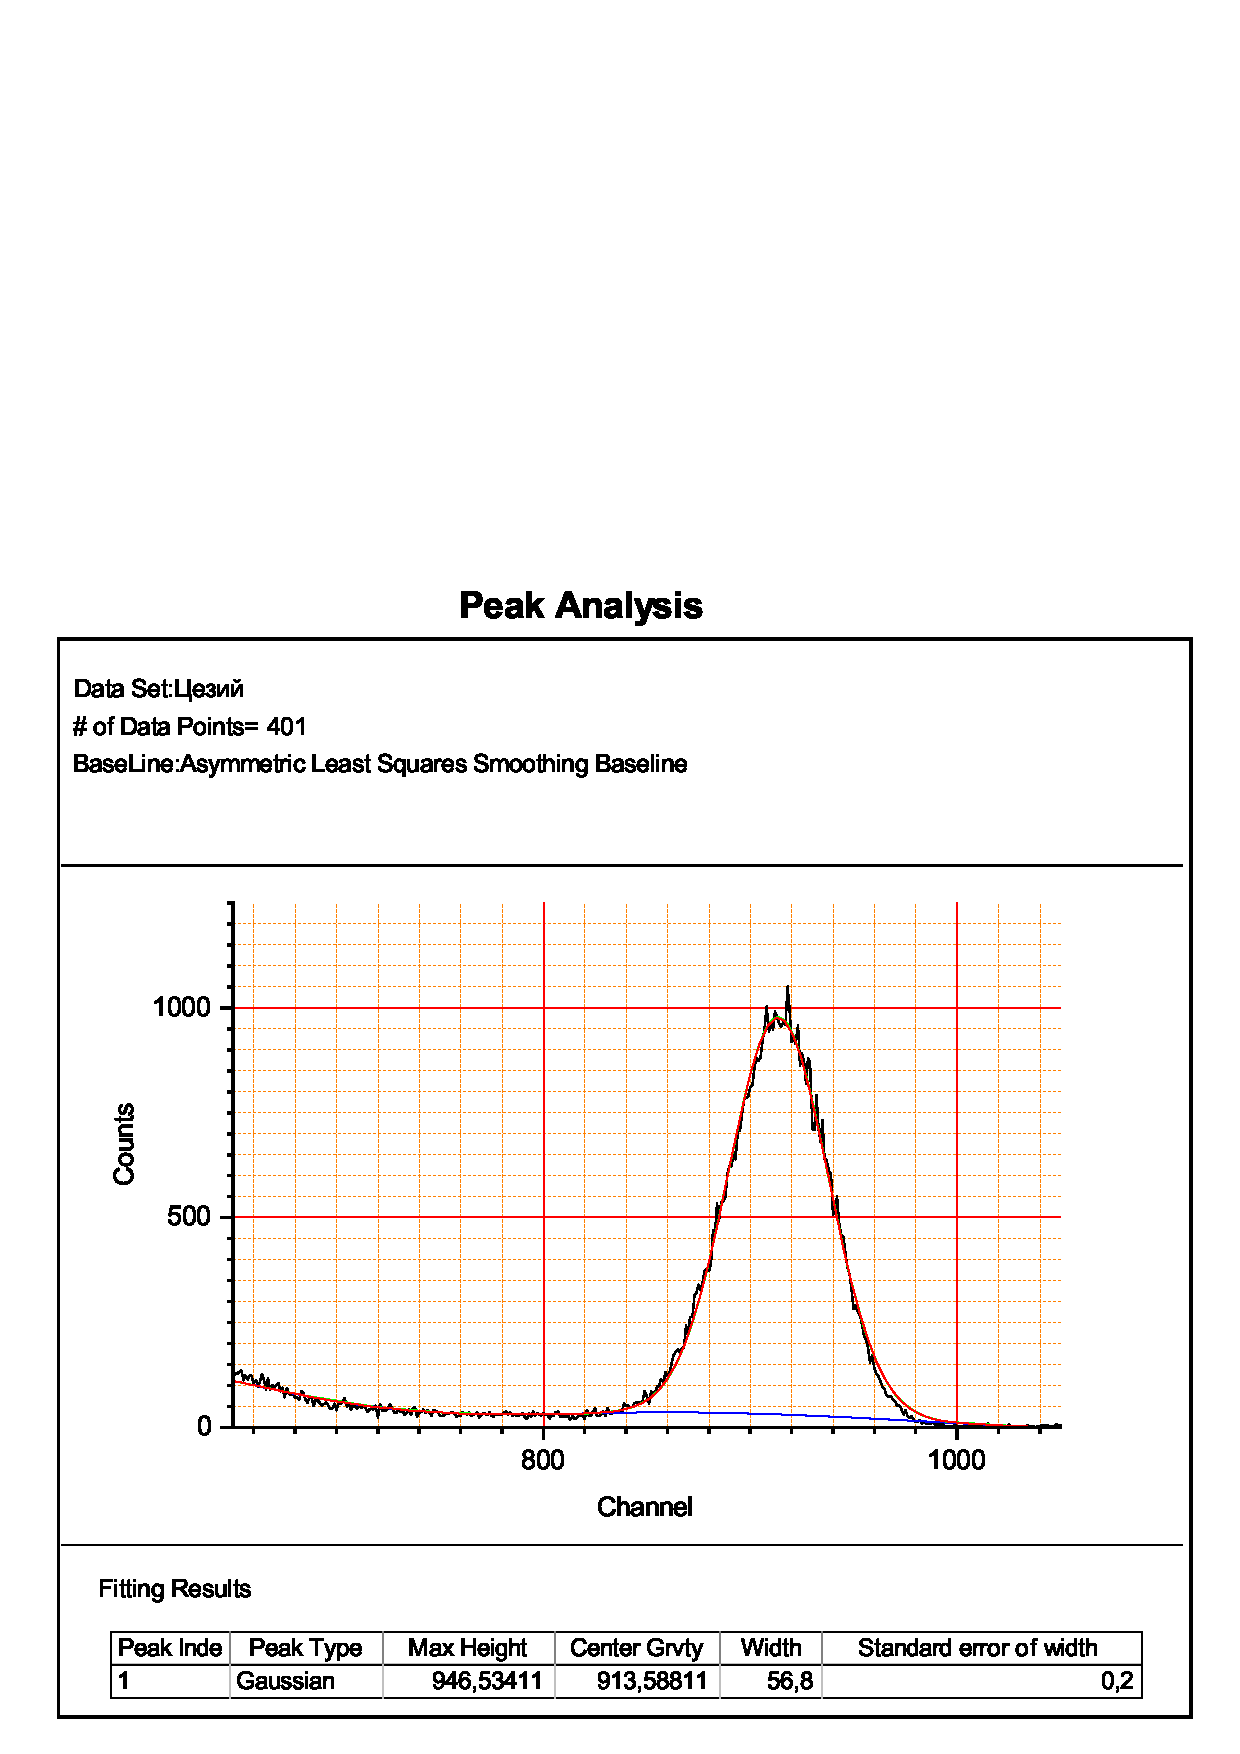
\includegraphics[width=0.8\linewidth]{3.jpg}\\
 
   \\
 
 \end{center}
 
 Данное явление происходит потому что отношение частот в струне и в генераторе отличаются в 2 раза. 


\subsection{†. Определение добротности Q струны как колебательной системы}


Измерим её амплитудно-частотную характеристику (АЧХ) вблизи одной из резонансных частот -- $\nu_1$ 
 
\begin{center}
\begin{tabular}{|c|c|}
	  \hline
 		$\nu, Гц$ & $А, у. е. $    \\
		\hline 
		238.4 & 1 \\
		\hline
		238.5 & 1.5\\
		\hline 
 		238.6 & 2.5\\
		\hline
 		238.7 & 4\\
		\hline
 		238.8 & 7\\
		\hline
		238.85 & 8\\
		\hline
 		238.9 & 4\\
		\hline
		239.0 & 2\\
		\hline
 		239.1 & 1.5\\
		\hline
		239.2 & 1\\
		\hline
	\end{tabular}
\end{center}


\begin{center}

  \includegraphics[width=0.8\linewidth]{task1.png}\\
 
   \\
 

 \end{center}
 Откуда можно найти добротность
  \begin{equation*}
  Q = \frac{\nu_1}{\Delta \nu} = 1200
  \end{equation*}

\section{Обсуждение результатов и выводы}

Теоретические и экспериментальные значения погонной плотности совпали в пределах погрешности, меньшей 5\%

\begin{equation*}
\frac{\Delta u}{u} &= \sqrt{(\frac{\Delta Т}{Т})^2+(\frac{\Delta \rho_l}{\rho_l})^2}= 0,5 \%\\
\end{equation*}


Так как для каждого измерения вращения использовалась серия измерений, то необходимо учитывать случайную погрешность.

\begin{equation*}
\sigma_{сл_u} &= \frac{1}{N}\sqrt{\sum\limits_{i=1}^n(u-\bar{u})} (в \ пределах \ до \ 0,5 \%)\\
\end{equation*}

Полная погрешность считается по формуле\\

\begin{align*}
\sigma &= \sqrt{\sigma_{сл}^2 +\sigma_{сист}^2} \\
\end{align*}

Откуда получаем выражение для погрешности для погонной плотности материала


\begin{align*}
\sigma_f &= \sqrt{\sigma_{сл}^2 + 4(\frac{\Delta u}{u})^2 +  (\frac{\Delta T}{T})^2 } = 4\% \\
\end{align*}




\end{document}
